\documentclass[aspectratio=169,11pt]{beamer}
\usepackage[utf8]{inputenc}
\usepackage[T1]{fontenc}
\usepackage[brazil]{babel}
\usepackage{lmodern}
\usepackage{amsmath,amssymb}
\usepackage{booktabs}
\usepackage{array}
\newcolumntype{L}[1]{>{\raggedright\arraybackslash}p{#1}}
\usepackage{graphicx}
\usepackage{listings}
\usepackage{tikz}
\usetikzlibrary{arrows.meta,positioning}

\graphicspath{{../relatorio/figuras/}}

% ---------- aparência ----------
\definecolor{azul}{HTML}{1F3A5F}
\definecolor{laranja}{HTML}{C8553D}
\definecolor{verde}{HTML}{2E7D4F}
\definecolor{cinza}{HTML}{6B7280}
\usetheme{default}
\setbeamercolor{frametitle}{fg=azul}
\setbeamercolor{title}{fg=azul}
\setbeamercolor{structure}{fg=azul}
\setbeamercolor{alerted text}{fg=laranja}
\setbeamercolor{block title}{bg=azul,fg=white}
\setbeamercolor{block body}{bg=azul!6}
\setbeamercolor{block title alerted}{bg=laranja,fg=white}
\setbeamercolor{block body alerted}{bg=laranja!7}
\setbeamercolor{block title example}{bg=verde,fg=white}
\setbeamercolor{block body example}{bg=verde!7}
\setbeamerfont{frametitle}{series=\bfseries,size=\Large}
\setbeamertemplate{navigation symbols}{}
\setbeamertemplate{itemize items}[circle]
\setbeamertemplate{blocks}[rounded]
\setbeamertemplate{footline}{%
  \hbox{\hspace{1em}\color{cinza}\tiny Diferenciação automática e passo complexo
  \hfill\insertframenumber/\inserttotalframenumber\hspace{1em}}\vspace{0.6em}}
\setbeamertemplate{section page}{%
  \centering\vfill{\color{cinza}\small \partelabel\ $\cdot$ Seção \insertsectionnumber}\\[0.4em]
  {\usebeamerfont{title}\color{azul}\Huge\bfseries\insertsectionhead}\vfill}
\newcommand{\partelabel}{}
\newcommand{\parte}[3]{%
  \renewcommand{\partelabel}{#1}%
  {\setbeamercolor{background canvas}{bg=azul}
  \begin{frame}[plain,noframenumbering]
    \centering\vfill
    {\color{white!70!azul}\large #1}\\[0.6em]
    {\color{white}\fontsize{34}{40}\selectfont\bfseries #2}\\[1em]
    {\color{white!80!azul}\normalsize #3}
    \vfill
  \end{frame}}}
\AtBeginSection{\begin{frame}[plain,noframenumbering]\sectionpage\end{frame}}

\lstset{language=Python, basicstyle=\ttfamily\footnotesize, keywordstyle=\color{azul}\bfseries,
  commentstyle=\color{verde}, stringstyle=\color{laranja}, columns=fullflexible,
  showstringspaces=false,
  literate={á}{{\'a}}1 {é}{{\'e}}1 {í}{{\'i}}1 {ó}{{\'o}}1 {ú}{{\'u}}1 {ã}{{\~a}}1
           {õ}{{\~o}}1 {ç}{{\c c}}1 {ê}{{\^e}}1 {â}{{\^a}}1 {ε}{{$\varepsilon$}}1 {²}{{$^2$}}1 {·}{{$\cdot$}}1}

\newcommand{\fl}{\operatorname{fl}}
\renewcommand{\Im}{\operatorname{Im}}
\renewcommand{\Re}{\operatorname{Re}}

\title{Diferenciação automática, passo complexo\\e diferenças finitas}
\subtitle{Por que só os dois primeiros atingem o arredondamento unitário}
\author{Felipe M. Figueira \and Lucas Carvalhosa Lago}
\date{Seminário --- 2026}

\begin{document}

\begin{frame}[plain,noframenumbering]
  \titlepage
\end{frame}

% =====================================================================
\parte{Parte I}{Teoria}{Por que diferenças finitas param antes de $u$, e como passo complexo e AD chegam lá}

% =====================================================================
\section{Motivação}

% =====================================================================
\begin{frame}{A pergunta central}
  \begin{block}{}
    \centering\large
    Por que diferenças finitas \alert{nunca} atingem erro $u$,\\
    e o que exatamente o passo complexo e a AD fazem para atingi-lo?\\[0.5em]
    \normalsize Qual é o custo em \textbf{generalidade} e em \textbf{implementação}?
  \end{block}
  \vspace{1em}
  \begin{columns}[T]
    \column{0.5\textwidth}
    Quatro formas de obter derivadas:
    \begin{enumerate}
      \item derivação manual
      \item derivação simbólica
      \item \alert{diferenças finitas}
      \item \alert{diferenciação automática (AD)}
    \end{enumerate}
    \column{0.45\textwidth}
    \textbf{Ponte entre 3 e 4:} o passo complexo (Squire--Trapp 1998; Martins et al.\ 2003).
    \vspace{0.6em}

    Usos: Newton, otimização, sensibilidade, redes neurais.
  \end{columns}
\end{frame}

% =====================================================================
\begin{frame}{Ponto de partida: derivada e série de Taylor}
  \begin{block}{Definição de derivada}
    \centering
    $\displaystyle f'(x) = \lim_{h\to0}\frac{f(x+h)-f(x)}{h}$
  \end{block}
  \begin{block}{Série de Taylor de $f$ em torno de $x$}
    \[
      f(x+h) = \sum_{k=0}^{\infty}\frac{f^{(k)}(x)}{k!}\,h^k
      = f(x) + hf'(x) + \frac{h^2}{2}f''(x) + \frac{h^3}{6}f'''(x) + \cdots
    \]
    Truncada em $n$ termos, com resto de Lagrange:
    \[
      f(x+h) = \sum_{k=0}^{n}\frac{f^{(k)}(x)}{k!}\,h^k + \frac{f^{(n+1)}(\xi)}{(n+1)!}\,h^{n+1},\qquad \xi\text{ entre } x \text{ e } x+h.
    \]
  \end{block}
  {\small A mesma expansão aparece em todo o seminário, só muda o \emph{passo}:
  $h$ real (diferenças finitas), $ih$ (passo complexo) e $b\,\varepsilon$ (números duais).}
\end{frame}

% =====================================================================
\begin{frame}{Modelo de ponto flutuante (IEEE-754)}
  Para números de máquina $a,b$ e $\circ\in\{+,-,\times,/\}$:
  \[
    \fl(a\circ b) = (a\circ b)(1+\delta),\qquad |\delta|\le u = 2^{-53}\approx 1{,}11\times10^{-16}.
  \]
  \begin{itemize}
    \item Avaliar $f$ custa um erro relativo da ordem de $u$:\quad $\hat f(x) = f(x)(1+\delta_f)$.
    \item Isso é o \textbf{piso}: nenhum método em precisão dupla faz, em geral, melhor que $\sim u$.
    \item Meta: um método de derivação cujo erro seja da \emph{mesma ordem} que o erro de avaliar $f$.
  \end{itemize}
\end{frame}

% =====================================================================
\section{Diferenças finitas}

% =====================================================================
\begin{frame}{Diferença progressiva e diferença centrada}
  \begin{columns}[c]
    \column{0.56\textwidth}
    \textbf{Progressiva} (troca o limite por um $h$ fixo):
    \[
      D_+(h) = \frac{f(x+h)-f(x)}{h} = f'(x) + \frac{h}{2}f''(\xi)
    \]
    Truncamento $O(h)$: ordem $p=1$.
    \vspace{0.6em}

    \textbf{Centrada}: subtraindo as séries de $f(x+h)$ e $f(x-h)$, os termos pares se cancelam.
    \column{0.42\textwidth}
    \centering
    \begin{tikzpicture}[scale=1.15, every node/.style={font=\scriptsize}]
      \draw[->,cinza] (-0.2,0) -- (4.2,0);
      \draw[->,cinza] (0,-0.2) -- (0,3.2);
      \draw[thick,azul,domain=0.2:4,smooth,samples=60] plot (\x,{0.18*\x*\x+0.2});
      % pontos x-h, x, x+h  (x=2, h=1.2)
      \foreach \t/\lab in {0.8/{x-h},2/{x},3.2/{x+h}}{
        \fill[azul] (\t,{0.18*\t*\t+0.2}) circle (1.3pt);
        \draw[cinza,dashed] (\t,0) -- (\t,{0.18*\t*\t+0.2});
        \node[below] at (\t,0) {$\lab$};
      }
      % tangente em x=2: inclinação 0.72
      \draw[verde,thick] (0.6,{0.92-0.72*1.4}) -- (3.6,{0.92+0.72*1.6});
      % secante progressiva: (2,0.92)-(3.2,2.0432), incl 0.936
      \draw[laranja,thick] (1.6,{0.92-0.936*0.4}) -- (3.7,{0.92+0.936*1.7});
      % secante centrada: (0.8,0.3152)-(3.2,2.0432), incl 0.72 (paralela à tangente)
      \draw[azul!70,very thick,dashed] (0.5,{0.3152-0.72*0.3}) -- (3.5,{0.3152+0.72*2.7});
      \node[verde,anchor=west] at (0.1,3.0) {tangente: $f'(x)$};
      \node[laranja,anchor=west] at (0.1,2.7) {secante progressiva};
      \node[azul!70,anchor=west] at (0.1,2.4) {secante centrada};
    \end{tikzpicture}
  \end{columns}
  \[
    D_c(h) = \frac{f(x+h)-f(x-h)}{2h} = f'(x) + \frac{h^2}{6}f'''(x) + \frac{h^4}{120}f^{(5)}(x) + \cdots
  \]
  Truncamento $O(h^2)$: ordem $p=2$, com o mesmo número de avaliações de $f$ (duas).
  {\small Para uma parábola a secante centrada é paralela à tangente: a centrada é exata.}
\end{frame}

% =====================================================================
\begin{frame}{Nota: cancelamento catastrófico}
  \begin{block}{O que é}
    Subtrair dois números \textbf{próximos} que já carregam erro de arredondamento. A subtração em si é exata (lema de Sterbenz), mas os dígitos iguais se anulam e sobram só os dígitos finais, justamente os contaminados:
    \[
      \frac{|\Delta(a-b)|}{|a-b|} \approx \frac{u\,(|a|+|b|)}{|a-b|} \;\gg\; u \quad\text{quando } a\approx b.
    \]
  \end{block}
  \vspace{0.2em}
  \begin{columns}[T]
    \column{0.52\textwidth}
    \textbf{Exemplo} ($e^x$ em $x=1$, $h=10^{-10}$):\\[0.2em]
    {\small\ttfamily
    \ \ 2,718281828\alert{7308734}\\
    $-$\,2,718281828\alert{4590450}\\
    = 0,000000000\alert{2718283}}\\[0.3em]
    {\small 10 dígitos se cancelam: a derivada sai com erro relativo $5\times10^{-7}$, não $10^{-16}$.}
    \column{0.44\textwidth}
    \begin{alertblock}{Por que importa aqui}
      Toda diferença finita \emph{precisa} subtrair $f(x+h)$ e $f(x)$, que ficam mais próximos quanto menor $h$. O erro $u|f|$ de cada valor vira $u|f|/h$ na derivada: é esse termo que impede chegar a $u$.
    \end{alertblock}
  \end{columns}
\end{frame}

% =====================================================================
\begin{frame}{Diferença progressiva: duas fontes de erro}
  Por Taylor:
  \[
    D_+(h) = \frac{f(x+h)-f(x)}{h} = f'(x) + \underbrace{\tfrac{h}{2}f''(\xi)}_{\text{truncamento}}
  \]
  Em ponto flutuante, cada $f$ tem erro absoluto $\le u|f|$, e $f(x+h)\approx f(x)$:
  \[
    |\hat D_+(h)-f'(x)| \lesssim \frac{h}{2}|f''| + \alert{\frac{2u|f|}{h}}
  \]
  \begin{alertblock}{Cancelamento catastrófico (nota anterior)}
    Truncamento cai com $h$; o termo de cancelamento cresce. Há um $h$ ótimo:
  \end{alertblock}
  \[
    h^\ast = 2\sqrt{u|f|/|f''|},\qquad E(h^\ast) = 2\sqrt{u|f||f''|} = O(u^{1/2})
  \]
\end{frame}

% =====================================================================
\begin{frame}{Extrapolação de Richardson}
  Ideia: o erro da centrada tem forma conhecida, $D_c(h) = f'(x) + a\,h^2 + b\,h^4 + \cdots$,
  com $a=\tfrac{f'''}{6}$ e $b=\tfrac{f^{(5)}}{120}$. Combinando dois passos:
  \[
    \begin{aligned}
      D_c(h)   &= f'(x) + a\,h^2 + b\,h^4 + \cdots\\
      D_c(h/2) &= f'(x) + \tfrac14 a\,h^2 + \tfrac1{16} b\,h^4 + \cdots
    \end{aligned}
  \]
  \[
    D_R(h) = \frac{4D_c(h/2)-D_c(h)}{3} = f'(x) - \frac{h^4}{480}f^{(5)}(x) + O(h^6)
  \]
  \begin{columns}[T]
    \column{0.48\textwidth}
    \begin{exampleblock}{Ganho}
      O termo $h^2$ some: ordem $p=4$ usando só valores de $D_c$.
    \end{exampleblock}
    \column{0.48\textwidth}
    \begin{alertblock}{Preço}
      Os coeficientes amplificam o arredondamento:
      $\tfrac43\cdot\tfrac{2u|f|}{h} + \tfrac13\cdot\tfrac{2u|f|}{2h} = \tfrac{3u|f|}{h}$.
    \end{alertblock}
  \end{columns}
  \[
    E_R(h)\approx \frac{h^4}{480}|f^{(5)}| + \frac{3u|f|}{h},\qquad
    h^\ast = \Big(\frac{360\,u|f|}{|f^{(5)}|}\Big)^{1/5},\qquad E_R(h^\ast) = O(u^{4/5}).
  \]
\end{frame}

% =====================================================================
\begin{frame}{Aumentar a ordem só ajuda até certo ponto}
  \renewcommand{\arraystretch}{1.5}
  \centering
  \begin{tabular}{lccc}
    \toprule
    Fórmula & erro total $E(h)$ & $h^\ast$ & melhor erro \\
    \midrule
    progressiva & $\frac{h}{2}|f''| + \frac{2u|f|}{h}$ & $\sim u^{1/2}$ & $O(u^{1/2})$ \\
    centrada & $\frac{h^2}{6}|f'''| + \frac{u|f|}{h}$ & $\sim u^{1/3}$ & $O(u^{2/3})$ \\
    Richardson & $\frac{h^4}{480}|f^{(5)}| + \frac{3u|f|}{h}$ & $\sim u^{1/5}$ & $O(u^{4/5})$ \\
    \bottomrule
  \end{tabular}
  \vspace{1em}

  \begin{block}{Observação: resultado geral (supondo $f^{(p+1)}(x)\ne0$)}
    Ordem $p$: \ $E(h)\approx C_ph^p + K_p\,u|f|/h$ \ $\Rightarrow$ \ $h^\ast\sim u^{1/(p+1)}$, \ $E(h^\ast)\sim u^{p/(p+1)}$.
    \\[0.3em]
    Como $p/(p+1)<1$, \alert{nenhuma} fórmula de ordem finita chega a $O(u)$.
  \end{block}
\end{frame}

% =====================================================================
\begin{frame}{De onde vem o $u/h$? Da subtração obrigatória}
  \small
  \textbf{Forma geral:} combinação de valores de $f$ em pontos $x+kh$, dividida por $h$: \quad $D(h) = \dfrac1h\displaystyle\sum_k c_k\,f(x+kh)$.
  \vspace{0.3em}
  \begin{columns}[T]
    \column{0.5\textwidth}
    \renewcommand{\arraystretch}{1.15}
    \begin{tabular}{lcc}
      \toprule
      fórmula & pontos $k$ & pesos $c_k$ \\
      \midrule
      progressiva & $0,\,1$ & $-1,\ 1$ \\
      centrada & $-1,\,1$ & $-\tfrac12,\ \tfrac12$ \\
      \bottomrule
    \end{tabular}
    \column{0.47\textwidth}
    \textbf{Duas condições} (Taylor em cada ponto):
    \begin{itemize}
      \item $\sum_k c_k = 0$: se $f$ é constante, $f'=0$, então os pesos devem se anular.
      \item $\sum_k k\,c_k = 1$: para sobrar exatamente $f'(x)$.
    \end{itemize}
  \end{columns}
  \vspace{0.3em}
  \begin{alertblock}{Consequência de $\sum_k c_k = 0$}
    Há pesos positivos e negativos: \textbf{subtraímos} valores $f(x+kh)\approx f(x)$. Cada valor tem erro $\approx u|f|$, e esses erros não se cancelam; divididos por $h$:
    \ $\text{erro de arredondamento}\approx \big(\textstyle\sum_k|c_k|\big)\,\dfrac{u|f|}{h}$.
  \end{alertblock}
  {\footnotesize Truncamento cai com $h$ (inclinação $+p$ em log-log); esse termo cresce (inclinação $-1$). Se $h$ ficar abaixo de meio ulp de $x$, $\fl(x+h)=x$ e a fórmula dá \textbf{zero}.}
\end{frame}

% =====================================================================
\section{Passo complexo}

% =====================================================================
\begin{frame}{Dedução (A1)}
  Se $f$ é real no eixo real e analítica perto de $x$:
  \[
    f(x+ih) = f(x) + ihf'(x) - \frac{h^2}{2}f''(x) - i\frac{h^3}{6}f'''(x) + \frac{h^4}{24}f^{(4)}(x) + \cdots
  \]
  Separando partes real e imaginária:
  \begin{align*}
    \Im f(x+ih) &= hf'(x) - \tfrac{h^3}{6}f'''(x) + O(h^5)\\
    \Re f(x+ih) &= f(x) - \tfrac{h^2}{2}f''(x) + O(h^4)
  \end{align*}
  \begin{block}{}
    \centering
    $\displaystyle f'(x) = \frac{\Im f(x+ih)}{h} + \frac{h^2}{6}f'''(x) + O(h^4)$
  \end{block}
  Truncamento $O(h^2)$, igual ao da centrada em módulo e com sinal oposto\\
  ({\small $h=10^{-3}$: $\mp 9{,}472\times10^{-6}$ de erro absoluto nos dois métodos}).
\end{frame}

% =====================================================================
\begin{frame}{Por que não aparece o termo $u/h$}
  \small
  \begin{columns}[T]
    \column{0.48\textwidth}
    \textbf{Centrada}: \ $\dfrac{\alert{f(x+h)-f(x-h)}}{2h}$
    \begin{itemize}
      \item dois números de tamanho $|f|$
      \item resultado de tamanho $2h|f'|$
      \item erro absoluto $u|f|$ vira erro relativo $u|f|/(h|f'|)$
    \end{itemize}
    \column{0.48\textwidth}
    \textbf{Passo complexo}: \ $\dfrac{\Im f(x+ih)}{h}$
    \begin{itemize}
      \item \textbf{nenhuma subtração}
      \item $hf'(x)$ \emph{é} a parte imaginária de um único número, com erro relativo $O(u)$
      \item dividir por $h$ não amplifica erro relativo
    \end{itemize}
  \end{columns}
  \vspace{0.3em}
  \begin{exampleblock}{Consequência}
    $E_{cs}(h)\approx \frac{h^2}{6}|f'''| + c\,u|f'|$. Para $h\lesssim 6{,}5\times10^{-9}$ o erro relativo de truncamento já é menor que $u$.
    \textbf{Não há compromisso}: $h=10^{-30}$ é uma escolha usual.
  \end{exampleblock}
\end{frame}

% =====================================================================
\begin{frame}{Segunda derivada pelo passo complexo (A3)}
  Da parte real de $f(x+ih)$:
  \[
    f(x)-\Re f(x+ih) = \frac{h^2}{2}f''(x) - \frac{h^4}{24}f^{(4)}(x)+\cdots
    \quad\Longrightarrow\quad
    f''(x)\approx\frac{2\,[\alert{f(x)-\Re f(x+ih)}]}{h^2}
  \]
  \begin{itemize}
    \item A subtração \textbf{volta}: dois números de tamanho $|f|$ que diferem em $O(h^2)$, cada um com erro $\sim u|f|$.
    \item Erro total: \ $E(h)\approx\dfrac{h^2}{12}|f^{(4)}| + \dfrac{4u|f|}{h^2}$ \ $\Rightarrow$ \ $h^\ast=\Big(\dfrac{48u|f|}{|f^{(4)}|}\Big)^{1/4}\sim u^{1/4}$, \ $E(h^\ast)\sim u^{1/2}$.
    \item É o mesmo balanço da centrada de 2ª ordem $\frac{f(x+h)-2f(x)+f(x-h)}{h^2}$.
  \end{itemize}
  \begin{block}{Por que o truque funciona para $f'$ e não para $f''$}
    Na parte imaginária, o primeiro termo \emph{já é} $hf'$: nada a remover. Na parte real, $\tfrac{h^2}{2}f''$ vem atrás de $f(x)$, e removê-lo exige subtrair.
  \end{block}
\end{frame}

% =====================================================================
\begin{frame}{E se o passo for inclinado?}
  Com passo puramente imaginário, só $f'$ sai livre de cancelamento. Mas o passo pode ser \textbf{inclinado}: $\omega = e^{i\pi/4}$, com $\omega^2=i$.
  \[
    \frac{\Im\big[f(x+\omega h) + f(x-\omega h)\big]}{h^2} = f''(x) - \frac{h^4}{360}f^{(6)}(x) + \cdots
  \]
  {\small (Lai e Crassidis, 2008)}
  \vspace{0.4em}
  \begin{columns}[T]
    \column{0.9\textwidth}
    \begin{itemize}
      \item Não subtrai termos $O(1)$ como $f(x)$.
      \item Ainda cancela termos $O(h)$: os $\pm hf'/\sqrt2$.
      \item Melhora muito, mas \alert{não chega a $u$}.
    \end{itemize}
  \end{columns}
  \vspace{0.6em}
  Derivadas superiores com erro $u$: várias unidades independentes (multicomplexos) ou hiperduais.
\end{frame}

% =====================================================================
\section{Números duais e AD}

% =====================================================================
\begin{frame}{A álgebra dos duais (A2)}
  $\mathbb D = \{a+b\varepsilon\}$ com \alert{$\varepsilon^2=0$}, \ $\varepsilon\ne0$.
  \vspace{0.4em}
  \begin{columns}[T]
    \column{0.46\textwidth}
    \textbf{Produto}
    \[ (a+b\varepsilon)(c+d\varepsilon) = ac + (ad+bc)\varepsilon \]
    Com $a=p(x),\ b=p'(x),\ c=q(x),\ d=q'(x)$:\\
    parte dual $= pq'+p'q = (pq)'$.\\
    \alert{Regra do produto.}
    \vspace{0.6em}

    \textbf{Quociente}
    \[ \frac{a+b\varepsilon}{c+d\varepsilon} = \frac ac + \frac{bc-ad}{c^2}\varepsilon \]
    \column{0.50\textwidth}
    \textbf{Funções elementares}
    \[ g(a+b\varepsilon) = \sum_k \tfrac{g^{(k)}(a)}{k!}(b\varepsilon)^k = g(a)+g'(a)\,b\,\varepsilon \]
    A série termina \emph{exatamente}: sem resto.\\[0.3em]
    Com $a=p(x)$, $b=p'(x)$: parte dual $=(g\circ p)'(x)$.\\
    \alert{Regra da cadeia.}
  \end{columns}
\end{frame}

% =====================================================================
\begin{frame}{Programas inteiros: o modo direto}
  \begin{block}{Proposição}
    Execute o programa de $f$ com $v_0 = x + 1\cdot\varepsilon$. Cada variável intermediária vale $v_j + \dot v_j\varepsilon$ com $\dot v_j = \mathrm dv_j/\mathrm dx$. Em particular, a saída é $f(x)+f'(x)\varepsilon$.
  \end{block}
  \textbf{Prova por indução} na ordem de execução (cada $v_j$ só usa $v_i,v_k$ com $i,k<j$):
  \begin{enumerate}
    \item \textbf{Álgebra} (o que o computador faz): define-se
      $\phi(a+b\varepsilon,\,c+d\varepsilon) := \phi(a,c) + [\partial_1\phi\, b + \partial_2\phi\, d]\,\varepsilon$.
    \item \textbf{Cálculo} (o que queremos): pela regra da cadeia multivariável,
      $\dfrac{\mathrm dv_j}{\mathrm dx} = \partial_1\phi_j\,\dot v_i + \partial_2\phi_j\,\dot v_k$.
  \end{enumerate}
  Os dois coincidem. \alert{A aritmética dual aplica a regra da cadeia um nó de cada vez.}
  \vspace{0.4em}

  {\small Laços e \texttt{if} só escolhem \emph{quais} operações rodam: o resultado é a derivada do caminho percorrido. Ela só coincide com $f'(x)$ se o caminho for o mesmo numa vizinhança de $x$; senão a AD erra sem avisar (\texttt{if x == 0: return 0 else: return x} dá $0$ em vez de $1$).}
\end{frame}

% =====================================================================
\begin{frame}{O que a indução prova, e o que não prova}
  \begin{columns}[T]
    \column{0.48\textwidth}
    \begin{exampleblock}{Prova (exatidão algébrica)}
      Em \textbf{aritmética exata}, a parte dual de cada variável é exatamente $\mathrm dv_j/\mathrm dx$.
      \begin{itemize}
        \item É uma afirmação sobre a \emph{álgebra} $\varepsilon^2=0$.
        \item Não há $h$, então não há truncamento: o método não aproxima nada.
      \end{itemize}
    \end{exampleblock}
    \column{0.48\textwidth}
    \begin{alertblock}{Não prova (arredondamento)}
      Que o número calculado em \texttt{float64} seja exato.
      \begin{itemize}
        \item Cada operação na parte dual erra $O(u)$, como na própria $f$.
        \item O erro final é $O(u)\times$ o condicionamento do cálculo de $f'$: argumento \emph{separado}.
      \end{itemize}
    \end{alertblock}
  \end{columns}
  \vspace{0.6em}
  \begin{block}{}
    \centering Exato $\neq$ sem erro: \textbf{AD não tem erro de método}; o erro de máquina continua lá, do mesmo tamanho que ao avaliar $f$.
  \end{block}
\end{frame}

% =====================================================================
\begin{frame}{Erro dos duais}
  \begin{itemize}
    \item Não há $h$ \ $\Rightarrow$ \ não há truncamento.
    \item Não há subtração de valores de $f$ \ $\Rightarrow$ \ não há $u/h$.
    \item Cada operação na parte dual tem erro relativo $O(u)$, como a avaliação da própria $f$.
  \end{itemize}
  \vspace{0.6em}
  \begin{exampleblock}{Resultado}
    Erro da derivada da mesma ordem do erro de calcular $f$: $O(u)$ vezes um fator de condicionamento do cálculo da derivada.
  \end{exampleblock}
  \vspace{0.6em}
  \centering
  \begin{tikzpicture}[node distance=1.2cm, every node/.style={font=\small}]
    \node[draw=azul,rounded corners,fill=azul!8,minimum width=2.4cm] (x) {$x+1\cdot\varepsilon$};
    \node[draw=azul,rounded corners,fill=azul!8,right=of x,minimum width=2.4cm] (p) {programa de $f$};
    \node[draw=verde,rounded corners,fill=verde!10,right=of p,minimum width=2.4cm] (y) {$f(x)+f'(x)\,\varepsilon$};
    \draw[-Latex,thick,azul] (x) -- (p);
    \draw[-Latex,thick,azul] (p) -- (y);
  \end{tikzpicture}
\end{frame}

% =====================================================================
\begin{frame}{Passo complexo e dual: a mesma construção}
  Números $a+b\,\delta$ com $\delta^2=\sigma$. \ $\sigma=0$: duais. \ $\sigma=-1$: complexos.
  \[
    f(x+h\delta) = \underbrace{\Big[f + \sigma\tfrac{h^2}{2}f'' + \sigma^2\tfrac{h^4}{24}f^{(4)}+\cdots\Big]}_{\text{parte ``real''}}
    + \underbrace{\Big[h f' + \sigma\tfrac{h^3}{6}f''' + \sigma^2\tfrac{h^5}{120}f^{(5)}+\cdots\Big]}_{\text{coeficiente de }\delta}\delta
  \]
  \begin{columns}[T]
    \column{0.48\textwidth}
    \begin{exampleblock}{Duais ($\sigma=0$)}
      Só o primeiro termo de cada colchete sobrevive. Exatidão \textbf{estrutural}, sem depender de $h$.
    \end{exampleblock}
    \column{0.48\textwidth}
    \begin{block}{Complexos ($\sigma=-1$)}
      A série não termina: termos ímpares ``vazam'' para a parte imaginária. Com $h=10^{-30}$ o vazamento fica muito abaixo de $u$.
    \end{block}
  \end{columns}
  \vspace{0.5em}
  \centering
  \alert{O passo complexo é um ``quase dual''}: chega a $u$ pela escolha de $h$; o dual chega pela álgebra.
\end{frame}

% =====================================================================
\begin{frame}{Resumo: erro total $=$ truncamento $+$ arredondamento}
  \[
    E(h) \;\approx\; \underbrace{\textcolor{azul}{C\,h^p}}_{\text{truncamento}} \;+\; \underbrace{\textcolor{laranja}{K\,\frac{u|f|}{h}}}_{\text{cancelamento}} \;+\; \underbrace{\textcolor{cinza}{c\,u|f'|}}_{\text{piso: avaliar } f}
  \]
  \vspace{0.2em}
  \centering
  \renewcommand{\arraystretch}{1.35}
  \small\begin{tabular}{lccc>{\raggedright\arraybackslash}p{4.2cm}}
    \toprule
    Método & \textcolor{azul}{$Ch^p$} & \textcolor{laranja}{$Ku|f|/h$} & melhor erro & por quê \\
    \midrule
    diferenças finitas & sim & \alert{sim} & $u^{p/(p+1)}$ & subtração obrigatória ($\sum c_k=0$) \\
    passo complexo & sim, $O(h^2)$ & \textbf{não} & $\sim u$ & sem subtração; $h$ minúsculo zera o truncamento \\
    duais (AD) & \textbf{não} & \textbf{não} & $\sim u$ & $\varepsilon^2=0$: série finita, sem $h$ \\
    \bottomrule
  \end{tabular}
  \vspace{0.6em}

  \raggedright\small
  Truncamento é erro \emph{do método} (existe em aritmética exata); arredondamento é erro \emph{da máquina} (some com $u\to0$). Diminuir $h$ reduz o primeiro e aumenta o segundo.
\end{frame}

% =====================================================================
\begin{frame}{Modo direto $O(n)$ $\times$ modo reverso $O(1)$}
  \begin{columns}[T]
    \column{0.48\textwidth}
    \textbf{Modo direto} (FD, complexo, dual)
    \begin{itemize}
      \item Cada passada dá uma derivada direcional $\nabla f\cdot v$.
      \item Gradiente: $n$ direções $\Rightarrow$ custo $\approx n\cdot$custo$(f)$.
      \item Dual com sementes vetoriais: uma passada, mas $Ax$ passa de $n^2$ a $n^3$ operações.
      \item Calcula $Jv$: \textbf{uma coluna} por vez.
    \end{itemize}
    \column{0.48\textwidth}
    \textbf{Modo reverso}
    \begin{itemize}
      \item Ida: avalia $f$ e grava a ``fita''.
      \item Volta: propaga adjuntos $\bar v_i \mathrel{+}= \bar v_j\,\partial\phi_j/\partial v_i$, a partir de $\bar f=1$.
      \item Custo $\le c\cdot$custo$(f)$, $c\approx3$--$5$, \alert{independente de $n$}.
      \item Calcula $v^\top J$: \textbf{uma linha} por vez.
    \end{itemize}
  \end{columns}
  \vspace{0.8em}
  \begin{block}{}
    Para $f:\mathbb R^n\to\mathbb R$, $J$ tem $n$ colunas e \textbf{uma} linha. O preço do reverso é memória: a fita cresce com o número de operações.
  \end{block}
\end{frame}

% =====================================================================
\begin{frame}{Direto $\times$ reverso: passadas e memória}
  \centering\small
  \renewcommand{\arraystretch}{1.25}
  \begin{tabular}{>{\raggedright\arraybackslash}p{3.2cm}>{\raggedright\arraybackslash}p{4.6cm}>{\raggedright\arraybackslash}p{4.6cm}}
    \toprule
    & Modo direto (duais) & Modo reverso \\
    \midrule
    propaga & tangentes $\dot v=\mathrm dv/\mathrm dx$, da entrada para a saída & adjuntos $\bar v=\partial f/\partial v$, da saída para a entrada \\
    calcula por passada & uma coluna $Jv$ & uma linha $v^\top J$ \\
    gradiente de $f:\mathbb R^n\to\mathbb R$ & $n$ passadas (ou uma com $n$ direções) & 1 ida $+$ 1 volta \\
    custo & $\approx n\cdot$custo$(f)$ & $\le c\cdot$custo$(f)$, $c\approx3$--$5$ \\
    memória extra & $O(1)$ por variável (ou $O(n)$ com $n$ direções) & \alert{fita}: $O(\#\text{operações})$ \\
    vale a pena quando & poucas entradas, muitas saídas & muitas entradas, poucas saídas \\
    \bottomrule
  \end{tabular}
  \vspace{0.6em}

  \raggedright\small
  Para $f:\mathbb R^n\to\mathbb R^m$: direto custa $\propto n$, reverso $\propto m$. Redes neurais têm $m=1$ (a perda) e $n$ enorme: por isso usam o reverso.
\end{frame}

% =====================================================================
\parte{Parte II}{Experimentos}{O que o notebook mede, e se bate com a teoria}

% =====================================================================
\section{Implementação e generalidade}

% =====================================================================
\begin{frame}{Como os experimentos foram feitos}
  \begin{columns}[T]
    \column{0.52\textwidth}
    \begin{itemize}
      \item Notebook do Lucas: \texttt{Automatic\_Differentiation\_\allowbreak Revisado.ipynb}.
      \item \texttt{float64} em tudo ($u=2^{-53}$), salvo onde comparamos com \texttt{float32}.
      \item Referências com 60 dígitos (\texttt{mpmath}).
      \item Bibliotecas: NumPy (nossa \texttt{Dual}), JAX e PyTorch.
      \item Onde a curva é ruidosa, comparamos a previsão com a \textbf{mediana} perto de $h^\ast$, não com o mínimo.
    \end{itemize}
    \column{0.44\textwidth}
    \begin{exampleblock}{Função de teste principal}
      \centering $f(x) = \dfrac{e^x}{\cos^3x+\sin^3x}$,\qquad $x = 1{,}5$\\[0.3em]
      {\small (Squire e Trapp, 1998; Martins et al., 2003)}
    \end{exampleblock}
    \vspace{0.3em}
    {\small B1, B2: classe \texttt{Dual} e cinco funções \\ C1: erro $\times$ $h$ \\ A3: segunda derivada \\ C2, C3, D1: gradientes, JAX e PyTorch}
  \end{columns}
\end{frame}

% =====================================================================
\begin{frame}[fragile]{Implementação: a classe \texttt{Dual} (B1)}
\begin{columns}[T]
\column{0.56\textwidth}
\begin{lstlisting}
class Dual:
    def __init__(self, val, der=0.0):
        self.val = real_finito(val, "val")
        self.der = np.array(der, dtype=float)

    # (a+bε)(c+dε) = ac + (ad+bc)ε
    def __mul__(self, other):
        other = Dual.converter(other)
        return Dual(self.val * other.val,
            self.der * other.val
            + self.val * other.der)

# g(a+bε) = g(a) + g'(a)·b·ε
def aplicar(x, g, dg):
    if isinstance(x, Dual):
        return Dual(g(x.val), dg(x.val) * x.der)
    return g(x)
\end{lstlisting}
\column{0.42\textwidth}
\small
\textbf{Decisões de projeto}
\begin{itemize}
  \item \textbf{Valida em vez de convencionar}: \texttt{abs} em $0$, \texttt{log} de não positivo e $0^p$ com $p<1$ levantam exceção.
  \item \textbf{Sementes vetoriais}: \texttt{der} pode ser um vetor; $x_i+e_i\varepsilon$ dá as $n$ parciais numa passada.
\end{itemize}
\end{columns}
\end{frame}

% =====================================================================
\begin{frame}[fragile]{Passo complexo: uma linha de código (B2)}
\begin{lstlisting}
def deriv_complexa(f, x, h=1e-30):
    return f(x + 1j * h).imag / h
\end{lstlisting}
  \vspace{0.5em}
  \begin{itemize}
    \item O termo $-\tfrac{h^2}{2}f''$ vai para a parte \emph{real} e não interfere.
    \item Funciona em código existente: basta que ele aceite números complexos.
    \item \textbf{Observação:} se a própria derivada for mal condicionada (soma de parcelas grandes que se anulam), há cancelamento \emph{interno}. Isso é próprio do problema e afeta igualmente a AD.
    \item Cuidado com $h$ extremo ($10^{-200}$): qualquer operação que forme $h^2$ no caminho (módulo, $z\bar z$) dá \emph{underflow}.
  \end{itemize}
\end{frame}

% =====================================================================
\begin{frame}{Cinco funções de teste (B2)}
  \centering\small
  \renewcommand{\arraystretch}{1.25}
  \begin{tabular}{L{6.0cm}L{3.4cm}L{3.4cm}}
    \toprule
    Função & Passo complexo & Dual \\
    \midrule
    1. $e^x$, $x=1$ & $0$ & $0$ \\
    2. $\log x$, $x=2$ & $0$ & $0$ \\
    3. $e^{\sin x^2}$, $x=0{,}7$ & $2{,}2\times10^{-16}$ & $0$ \\
    4. $|x|$, $x=\pm1$ & \textcolor{laranja}{falha}: $0$ & correto ($\pm1$) \\
    \phantom{4.} $|x|$, $x=0$ (não diferenciável) & $0$, sem aviso & \texttt{ValueError} \\
    5. $[A(x)^{-1}r]_1$ via \texttt{np.linalg.solve}, $x=1$ & $-0{,}36$ (correto) & \textcolor{laranja}{falha} (\texttt{dtype=object}) \\
    \bottomrule
  \end{tabular}
  \vspace{0.6em}

  \raggedright
  Erros relativos nas funções 1--3: ambos chegam a $\sim u$. Na 4 o passo complexo falha \emph{longe} da singularidade; na 5 quem falha é a \texttt{Dual}.
\end{frame}

% =====================================================================
\begin{frame}{Função 4: \texttt{abs} apaga a derivada em silêncio}
  \begin{itemize}
    \item Para complexos, \texttt{abs} calcula o módulo $\sqrt{\Re^2+\Im^2}$, que é \textbf{real}.
    \item A parte imaginária (que carregava a derivada) é jogada fora.
    \item Resultado $0$ \alert{longe} do ponto singular ($x=\pm1$), sem nenhum aviso.
  \end{itemize}
  \begin{block}{Correção de Martins et al.\ (2003)}
    \centering $\mathrm{abs\_cs}(z) = \begin{cases}-z, & \Re z<0\\ \ \ z, & \text{caso contrário}\end{cases}$
  \end{block}
  \begin{itemize}
    \item Mesmas armadilhas: \texttt{max}/\texttt{min}, comparações, conjugação ($x\bar x$ no lugar de $x^2$).
    \item Em $x=0$, onde $f'$ não existe: passo complexo devolve $0$ em silêncio; a nossa \texttt{Dual} levanta \texttt{ValueError}.
    \item $\sqrt{x^2}$ em $0$: a AD faz $0/0$ na regra da cadeia, embora $\sqrt{x^2}=|x|$. A derivada depende do \emph{programa}.
  \end{itemize}
\end{frame}

% =====================================================================
\begin{frame}{Função 5: código compilado}
  \begin{columns}[T]
    \column{0.48\textwidth}
    \begin{exampleblock}{Passo complexo funciona}
      O LAPACK tem rotinas complexas (\texttt{zgesv}). A extensão analítica de $x\mapsto A(x)^{-1}b$ é a inversão em aritmética complexa.
    \end{exampleblock}
    \column{0.48\textwidth}
    \begin{alertblock}{\texttt{Dual} falha}
      \texttt{solve} converte a entrada num \texttt{ndarray} numérico. Nem \texttt{Dual} de matrizes nem matriz de \texttt{Dual}s (\texttt{dtype=object}) são tipos que o código compilado conheça.
    \end{alertblock}
  \end{columns}
  \vspace{0.8em}
  \textbf{Saída:} uma regra de derivada para a rotina inteira. De $My=r$:
  \[
    M\,\mathrm dy = \mathrm dr - \mathrm dM\,y \qquad\Longrightarrow\qquad \text{um segundo \texttt{solve} com a mesma } M.
  \]
  É assim que PyTorch e JAX tratam álgebra linear: o \texttt{autograd} traz uma regra pronta para \texttt{solve}, em vez de derivar o LAPACK por dentro.
\end{frame}

% =====================================================================
\section{Precisão: erro em função de $h$}

% =====================================================================
\begin{frame}{O ``V'' do erro (experimento C1)}
  \centering
  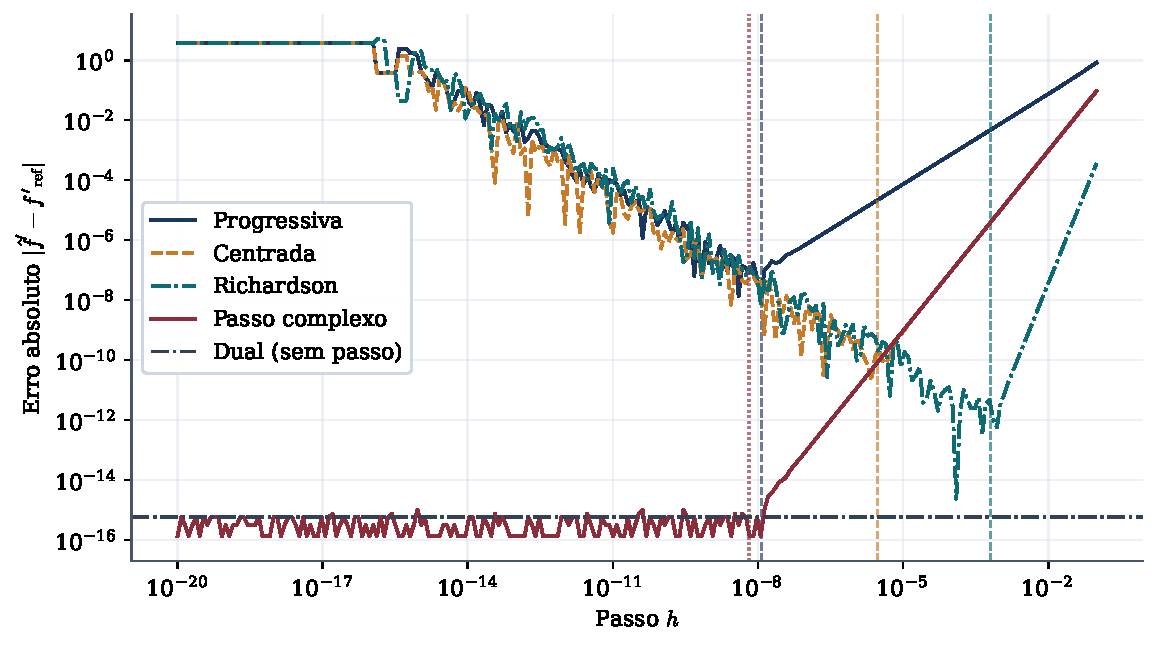
\includegraphics[height=0.78\textheight]{notebook_original/c1.pdf}\\
  \small Erro absoluto de $f'(1{,}5)$ para $h\in[10^{-20},10^{-1}]$, com passo efetivo $(x+h)-x$. Tracejado: $h^\ast$ do modelo; horizontal: \texttt{Dual}.
\end{frame}

% =====================================================================
\begin{frame}{Teoria $\times$ experimento}
  \centering
  \renewcommand{\arraystretch}{1.3}
  \begin{tabular}{lcccc}
    \toprule
    Método & $p$ & $h^\ast$ do modelo & erro previsto & mediana perto de $h^\ast$ \\
    \midrule
    progressiva & 1 & $1{,}2\times10^{-8}$ & $1{,}7\times10^{-7}$ & $9{,}8\times10^{-8}$ \\
    centrada & 2 & $3{,}0\times10^{-6}$ & $2{,}5\times10^{-10}$ & $9{,}5\times10^{-11}$ \\
    Richardson & 4 & $6{,}4\times10^{-4}$ & $2{,}9\times10^{-12}$ & $3{,}3\times10^{-12}$ \\
    \alert{passo complexo} & 2 & $h\lesssim6{,}5\times10^{-9}$ & $4{,}0\times10^{-16}$ & $3{,}1\times10^{-16}$ \\
    \alert{dual} & --- & --- & $\sim u|f'|$ & $5{,}8\times10^{-16}$ \\
    \bottomrule
  \end{tabular}

  {\footnotesize Erros absolutos; $f'(1{,}5)=3{,}622$. Mínimos isolados da malha (p.\,ex.\ $2{,}4\times10^{-15}$ em Richardson) são cancelamentos fortuitos.}
  \vspace{1em}
  \begin{itemize}
    \item As três diferenças finitas têm a \textbf{mesma perna esquerda} $u|f|/h$: aumentar a ordem só abaixa o vértice do ``V''.
    \item O passo complexo tem a perna direita da centrada, mas \alert{não tem perna esquerda}.
  \end{itemize}
\end{frame}

% =====================================================================


\begin{frame}{Segunda derivada: experimento (A3)}
  \begin{columns}[c]
    \column{0.56\textwidth}
    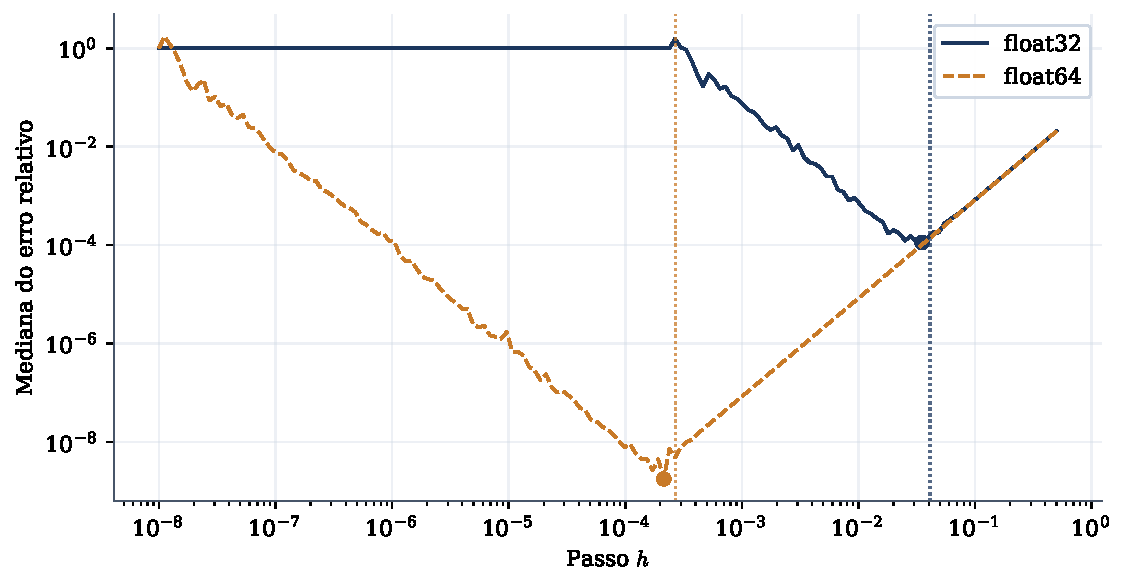
\includegraphics[width=\textwidth]{notebook_original/a3.pdf}
    \column{0.42\textwidth}
    \small
    $(e^x)''$ pela parte real do passo complexo, mediana em 65 pontos de $[0,1]$.
    \begin{itemize}
      \item Modelo: $h^\ast=(48u)^{1/4}$, erro $\sim2\sqrt{u/3}$.
      \item \texttt{float32}: $h^\ast$ previsto $4{,}1\times10^{-2}$; mínimo $1{,}1\times10^{-4}$ em $3{,}5\times10^{-2}$.
      \item \texttt{float64}: $h^\ast$ previsto $2{,}7\times10^{-4}$; mínimo $1{,}8\times10^{-9}$ em $2{,}1\times10^{-4}$.
      \item Razão dos $h$ ótimos: 163 medido, 152 previsto.
      \item O cancelamento volta: erro $\sim\sqrt u$, longe de $u$.
    \end{itemize}
  \end{columns}
\end{frame}

% =====================================================================
\section{Gradientes e bibliotecas}

% =====================================================================
\begin{frame}{Gradiente em $\mathbb R^{100}$ (C2)}
  $f(x) = \tfrac12x^\top Ax - b^\top x$, \ $A=M^\top M/n+I$ simétrica, \ $\nabla f = Ax - b$.
  \vspace{0.4em}

  \centering\small
  \renewcommand{\arraystretch}{1.25}
  \begin{tabular}{lccc}
    \toprule
    Método & avaliações & erro rel. & tempo (ms) \\
    \midrule
    diferenças centradas & 200 reais & $5{,}8\times10^{-10}$ & $15$ \\
    passo complexo & 100 complexas & $2{,}4\times10^{-16}$ & $73$ \\
    \texttt{Dual} vetorizada & 1 (100 direções) & $3{,}6\times10^{-16}$ & $359$ \\
    \texttt{torch.func.jacfwd} & 1 (vetorizada) & $9{,}5\times10^{-17}$ & --- \\
    \texttt{torch.func.grad} (reverso) & 1 direta + 1 reversa & $1{,}9\times10^{-16}$ & --- \\
    \bottomrule
  \end{tabular}
  \vspace{0.6em}

  \raggedright
  Como $f$ é quadrática, $f'''\equiv0$: os $6\times10^{-10}$ da centrada são \alert{puro cancelamento}. A \texttt{Dual} faz $O(n^3)$ operações, como o passo complexo, mas cada entrada de $Ax$ é um objeto Python: a lentidão é do interpretador, não do método.
\end{frame}

% =====================================================================
\begin{frame}{Na quadrática, a centrada só tem cancelamento (C2b)}
  \begin{columns}[c]
    \column{0.56\textwidth}
    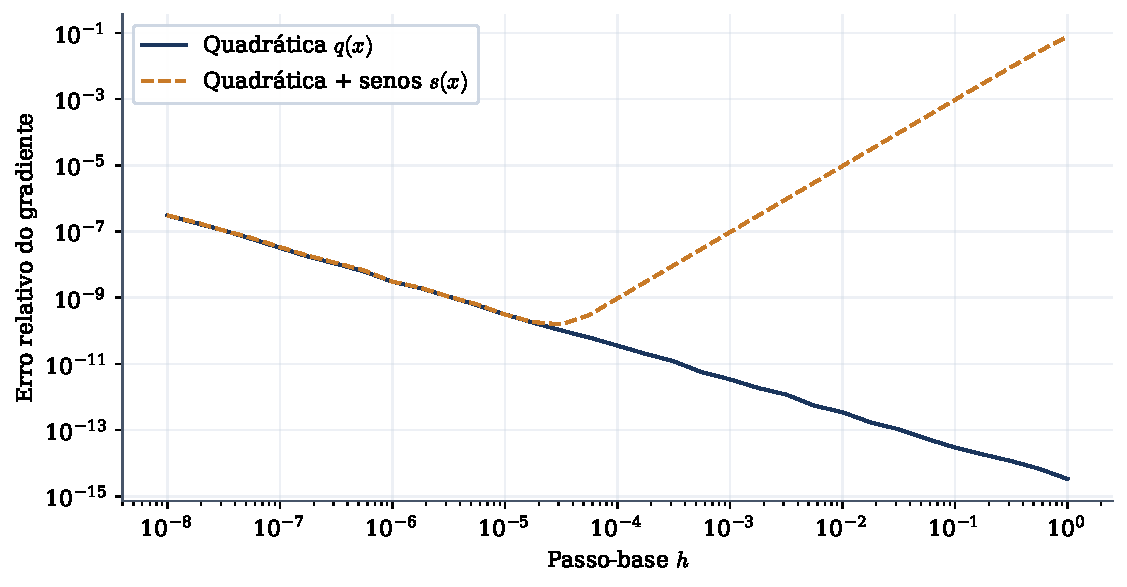
\includegraphics[width=\textwidth]{notebook_original/c2b.pdf}
    \column{0.42\textwidth}
    \small
    \begin{itemize}
      \item Quadrática: $f'''\equiv0$, sem truncamento. O erro cai até $3{,}3\times10^{-15}$ com $h=1$.
      \item Somando $\sum_i\sin x_i$: volta o ``V'', mínimo $1{,}6\times10^{-10}$ em $h\approx3\times10^{-5}$.
      \item Separa experimentalmente as duas fontes de erro.
    \end{itemize}
  \end{columns}
\end{frame}

% =====================================================================


% =====================================================================
\begin{frame}{JAX e PyTorch (C3, D1)}
  \small
  \begin{columns}[T]
    \column{0.5\textwidth}
    \textbf{Gradiente da quadrática ($n=100$)}\\[0.3em]
    \begin{tabular}{lc}
      \toprule
      método & erro rel. \\
      \midrule
      \texttt{jax.jacfwd} (direto) & $1{,}5\times10^{-16}$ \\
      \texttt{jax.grad} (reverso) & $1{,}7\times10^{-16}$ \\
      \texttt{torch.func.jacfwd} & $9{,}5\times10^{-17}$ \\
      \texttt{torch.func.grad} & $1{,}9\times10^{-16}$ \\
      \texttt{backward()} & $1{,}9\times10^{-16}$ \\
      \bottomrule
    \end{tabular}
    \column{0.46\textwidth}
    \textbf{Tempo em JAX} (mediana após aquecimento)\\[0.3em]
    \begin{tabular}{lcc}
      \toprule
      & sem JIT & com JIT \\
      \midrule
      direto & $4{,}4$\,ms & $0{,}23$\,ms \\
      reverso & $5{,}1$\,ms & $0{,}03$\,ms \\
      \bottomrule
    \end{tabular}\\[0.4em]
    Com JIT, o reverso foi $8\times$ mais rápido que o direto. Com $n=100$ só, isso ilustra a diferença, mas não mede um expoente.
  \end{columns}
  \vspace{0.6em}
  $(e^{\sin x^2})'(0{,}7)$: \texttt{Dual} $0$; passo complexo $4{,}4\times10^{-16}$; JAX e PyTorch $2{,}2\times10^{-16}$.
\end{frame}

% =====================================================================
\begin{frame}{Pontos não diferenciáveis: cada ferramenta escolhe (C3)}
  \begin{columns}[c]
    \column{0.48\textwidth}
    \centering
    \renewcommand{\arraystretch}{1.2}
    \begin{tabular}{lc}
      \toprule
      Cálculo em $x=0$ & resultado \\
      \midrule
      \texttt{jax.grad(jnp.abs)} & $1$ \\
      \texttt{torch.abs} (autograd) & $0$ \\
      passo complexo + \texttt{abs} & $0$ \\
      nossa \texttt{Dual} & \texttt{ValueError} \\
      \bottomrule
    \end{tabular}
    \column{0.48\textwidth}
    \begin{itemize}
      \item Subdiferencial de $|x|$ em $0$: $[-1,1]$.
      \item JAX: ramo $x\ge0$ (lateral direita).
      \item PyTorch: $\operatorname{sign}(0)=0$ (subgradiente de norma mínima).
      \item Passo complexo: $0$ porque \texttt{abs} apaga a parte imaginária; \texttt{Dual}: sinaliza.
    \end{itemize}
    \vspace{0.5em}
    \begin{alertblock}{Lição}
      AD devolve a derivada exata \emph{do programa no ramo executado}. Em pontos de quebra, o resultado é convenção, não matemática.
    \end{alertblock}
  \end{columns}
\end{frame}

% =====================================================================
\begin{frame}{Função $\times$ programa: derivadas em $x=0$}
  \centering\footnotesize
  \renewcommand{\arraystretch}{1.3}
  \begin{tabular}{lccccc}
    \toprule
    programa & $f'(0)$ real & passo complexo & nossa \texttt{Dual} & JAX & PyTorch \\
    \midrule
    $|x|$ & não existe & $0$ & \texttt{ValueError} & $1$ & $0$ \\
    $\sqrt{x\cdot x}$ \ ($=|x|$) & não existe & $1$ & \texttt{ValueError} & \texttt{nan} & \texttt{nan} \\
    \texttt{0 if x == 0 else x} \ ($=x$) & $1$ & $1$ & $0^\ast$ & $0$ & $0$ \\
    \bottomrule
  \end{tabular}
  \vspace{0.5em}

  \raggedright
  {\footnotesize $^\ast$ comparando pela parte real, como faz a AD. Valores medidos à parte em \texttt{float64}; só a linha de $|x|$ está no notebook.}
  \vspace{0.5em}
  \begin{itemize}
    \item As três linhas descrevem funções simples, mas cada \emph{programa} dá respostas diferentes.
    \item A AD deriva \textbf{o caminho executado}: no \texttt{if}, o ramo $x=0$ é a constante $0$, e a derivada sai $0$ embora $f(x)=x$.
    \item O passo complexo erra por outro motivo: $|x|$ apaga a parte imaginária; $x+ih\neq0$ pula o \texttt{if}.
    \item Em ponto de quebra, nenhum método ``descobre'' que a derivada não existe; no máximo, sinaliza.
  \end{itemize}
\end{frame}

% =====================================================================
\parte{Conclusões}{Conclusões}{}

% =====================================================================
\begin{frame}{Resumo comparativo}
  \centering\footnotesize
  \renewcommand{\arraystretch}{1.3}
  \begin{tabular}{L{2.2cm}L{2.2cm}L{2.8cm}L{2.8cm}L{2.6cm}}
    \toprule
    & Dif.\ finitas & Passo complexo & AD direta (duais) & AD reversa \\
    \midrule
    Melhor erro & $u^{p/(p+1)}$ & $\sim u$ & $\sim u$ & $\sim u$ \\
    Parâmetro $h$ & crítico & irrelevante ($h\ll\sqrt u$) & não há & não há \\
    Exige de $f$ & só avaliar & analítica, código \emph{complex-safe} & operações sobrecarregáveis & idem, mais fita \\
    Código compilado & sim & se aceitar complexos & só com regra própria & só com regra própria \\
    Gradiente em $\mathbb R^n$ & $n$ ou $2n$ aval. & $n$ aval.\ complexas & $n$ direções & $O(1)$ aval., memória $O(\#\text{ops})$ \\
    2ª derivada & cancelamento & cancelamento volta & exata (aninhado) & exata (aninhado) \\
    \bottomrule
  \end{tabular}
\end{frame}

% =====================================================================
\begin{frame}{Respostas à pergunta central}
  \begin{enumerate}
    \setlength{\itemsep}{0.6em}
    \item \textbf{Por que diferenças finitas nunca atingem $u$:} ser exata em constantes obriga a subtrair valores próximos de $f$; isso gera $u|f|/h$, e o equilíbrio com $Ch^p$ limita o erro a $u^{p/(p+1)}$.
    \item \textbf{Passo complexo:} empurra a perturbação para uma direção ``ortogonal'', onde $f'$ aparece isolada. Sem subtração, sem $u/h$; o truncamento some com $h$ minúsculo.
    \item \textbf{AD:} troca $i^2=-1$ por $\varepsilon^2=0$. A série de Taylor fica finita, não há truncamento, e o único erro é o arredondamento da própria aritmética.
    \item \textbf{O custo:} o passo complexo exige analiticidade e código \emph{complex-safe}, mas atravessa bibliotecas complexas. A AD exige que tudo passe pela sobrecarga (ou tenha regra própria), mas permite o modo reverso, o único com gradiente a custo $O(1)$. Nenhum resolve pontos não diferenciáveis.
  \end{enumerate}
\end{frame}

% =====================================================================
\begin{frame}{Referências}
  \small
  \begin{itemize}
    \item W.~Squire e G.~Trapp. Using complex variables to estimate derivatives of real functions. \emph{SIAM Review}, 40(1):110--112, 1998.
    \item J.~R.~R.~A. Martins, P.~Sturdza e J.~J. Alonso. The complex-step derivative approximation. \emph{ACM TOMS}, 29(3):245--262, 2003.
    \item A.~G. Baydin, B.~A. Pearlmutter, A.~A. Radul e J.~M. Siskind. Automatic differentiation in machine learning: a survey. \emph{JMLR}, 18(153):1--43, 2018.
    \item A.~Griewank e A.~Walther. \emph{Evaluating Derivatives}. 2.\,ed., SIAM, 2008.
    \item K.-L. Lai e J.~L. Crassidis. Extensions of the first and second complex-step derivative approximations. \emph{J. Comput. Appl. Math.}, 219:276--293, 2008.
    \item N.~J. Higham. \emph{Accuracy and Stability of Numerical Algorithms}. 2.\,ed., SIAM, 2002.
  \end{itemize}
  \vfill
  \centering\Large\color{azul}\textbf{Perguntas?}
\end{frame}

\end{document}
